Data augmentation is a technique for enlarging existing dataset with new samples created from already existing ones. There exist many techniques that allow us to do so. The more traditional ones focus on transformations of the original images. However, with the rise of artificial intelligence, generative techniques have emerged that allow us to generate artificial samples using deep learning models. In this work, we will focus on generative models that can create synthetic samples from Gaussian noise. 

% \begin{figure}[H]
%     \centering
%     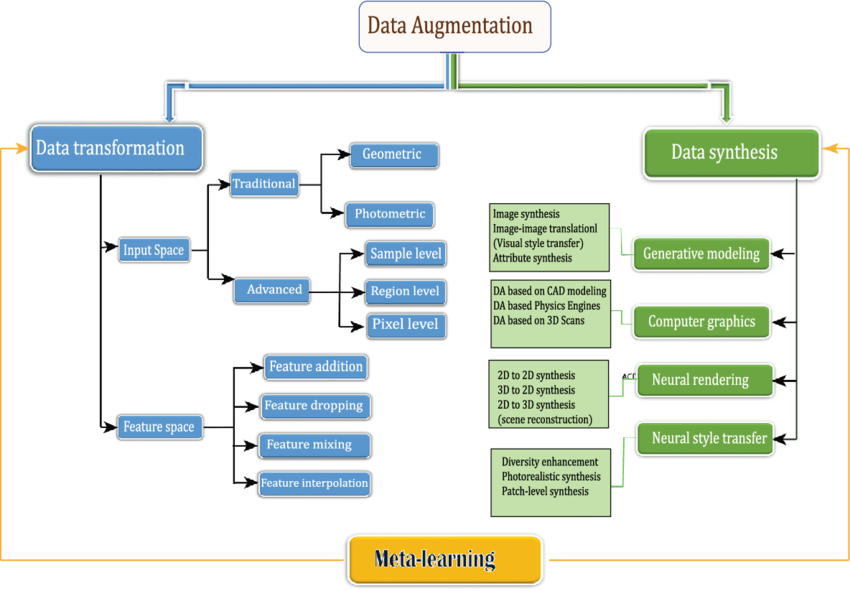
\includegraphics[width=0.99\linewidth]{background/Taxonomy-of-data-augmentation-approaches-used-in-this-survey.png}
%     \caption{Data augmentation taxonomy\cite{Mumuni2022-ka}.}
%     \label{fig:enter-label}
% \end{figure}

\begin{figure}[H]
    \centering
    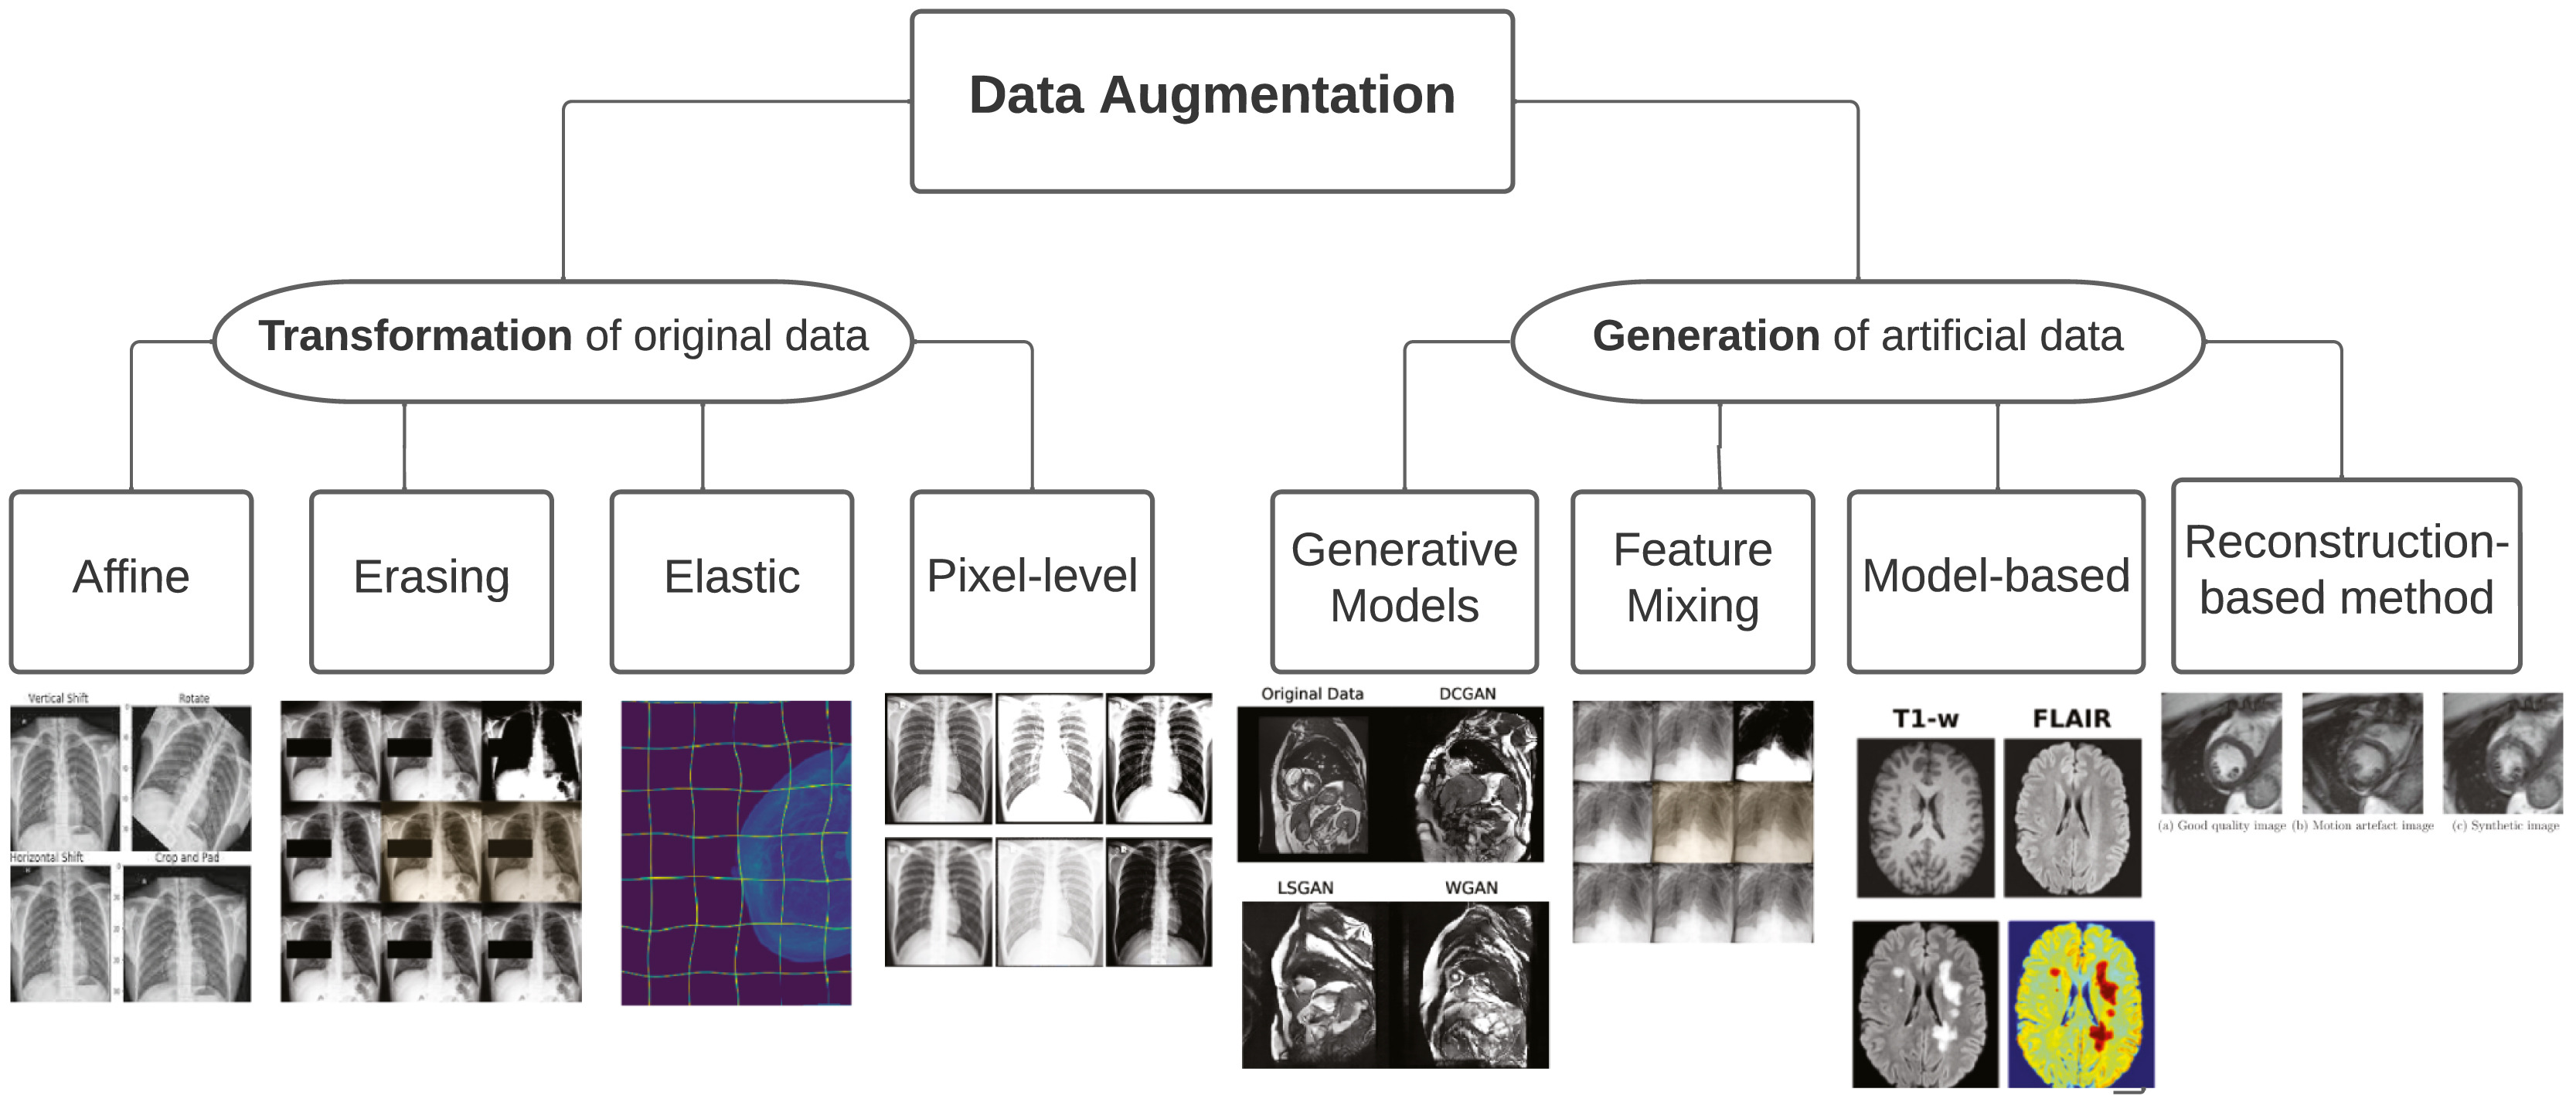
\includegraphics[width=0.99\linewidth]{background/taxonomy-data-augmentation.jpg}
    \caption{Data augmentation taxonomy\cite{GARCEA2023106391}.}
    \label{fig:enter-label}
\end{figure}

% The types of transformations
% \paragraph{Affine transformations} are geometric transformations that preserve lines and parallelism. They do not preserve angles and distances. Exemplary are: rotating, translating, scaling, horizontal and vertical shifting, cropping, padding, shearing.

% \paragraph{Erasing transformation} are used to replace some part of an image with some fixed value or random noise. 

% \paragraph{Pixel level}



\subsection{Generative Medical Imaging}
Medical imaging field in the AI landscape suffers from insufficient data. Thus scientists around the world started to explore generative networks. Now they are the most popular solution for the generation of medical images\cite{osuala2023data}.
Generative models provide a greater potential for data augmentation, in comparison to transformation techniques, by producing a wider variety of samples. However, these methods are much more complex and require significant computational resources.

Artificial samples obtained this way may not have the same visual characteristics or distribution as the original set. Additionally, the samples obtained in this way may include artifacts, even invisible to the human eye, that could be harmful to the models that would be trained on them.
\subsection{State of the art techniques for generative medical imaging}